% ############### 2.2) COMPONENT VIEW ####################
% sources:
% https://www.ibm.com/cloud/learn/microservices#toc-common-pat--cw3xiYi
% https://www.devteam.space/blog/microservice-architecture-examples-and-diagram/

% This architecture will follow some patterns for example:

% \begin{itemize}
%     \item Backend-for-frontend (BFF) pattern: This pattern inserts a layer between the user experience and the resources that experience calls on. This will allow to create and support one backend type per user interface using the best options for that interface, rather than trying to support a generic backend that works with any interface but may negatively impact frontend performance.
%     \item Entity and aggregate patterns: An entity is an object distinguished by its identity. An aggregate is a collection of related entities that should be treated as one unit. That allow to classify data in meaningful ways.
%     \item Adapter microservices patterns: The purpose of adapter patterns is to help translate relationships between classes or objects that are otherwise incompatible (for example for communication between application and thir party APIs).
% \end{itemize}

In order to reduce the complexity of the (cfr.\textbf{solution domain} \cite{bruegge2013object}, \S 6.3.2), the required functionalities of the software are here decomposed by solution domains classes. A domain is consists of multiple sub-domains. A sub-domain is a replaceable part of the system with well-defined interfaces that encapsulates the state and behavior of its contained classes. Each sub-domain corresponds to a different part of the business. By decomposing the system into relatively independent subsystems, concurrent teams can work on individual subsystems with minimal communication overhead. Some business functionalities require the aggregation of micro-services functionalities (\ie for processing complex queries about farmer's information). As described in section \ref{sec:styles_patterns}, the system should make use of the CQRS pattern to fulfill the above mentioned requirement. Here we provide the internal structure that the interested micro-service components should implement to achieve this task:


% (https://microservices.io/patterns/decomposition/decompose-by-subdomain.html)
\begin{figure}[H]
	\centering
    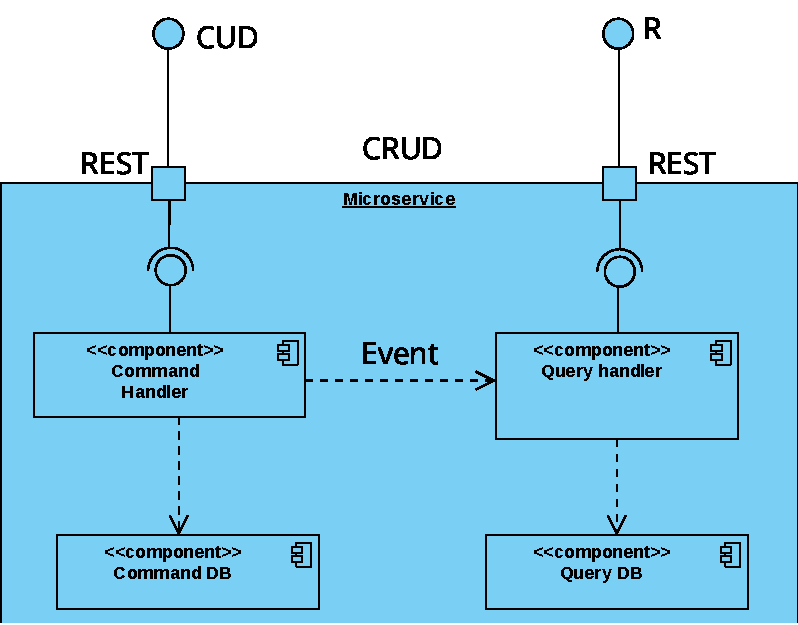
\includegraphics[ width=0.5\textwidth]{Images/CRUD_microservice.pdf}
	\caption{\label{fig:CRUD_microservice}CQRS-based micro-service}
\end{figure}


In a CQRS-based service (ref.\cite{richardson2018microservices}, \S7.2.2), the command-side domain module handles CRUD operations and is mapped to its own database. It handles simple queries, such as non join, primary key-based queries. The command side publishes domain events whenever its data changes. These events might be published using event sourcing. A separate query module handles simple queries. It’s much simpler than the
command side because it’s not responsible for implementing the business rules. The
query side uses whatever kind of database makes sense for the queries that it must support. The query side has event handlers that subscribe to domain events and update
the database.

The overall component diagram is shown below:


\begin{figure}[H]
    \makebox[\textwidth]{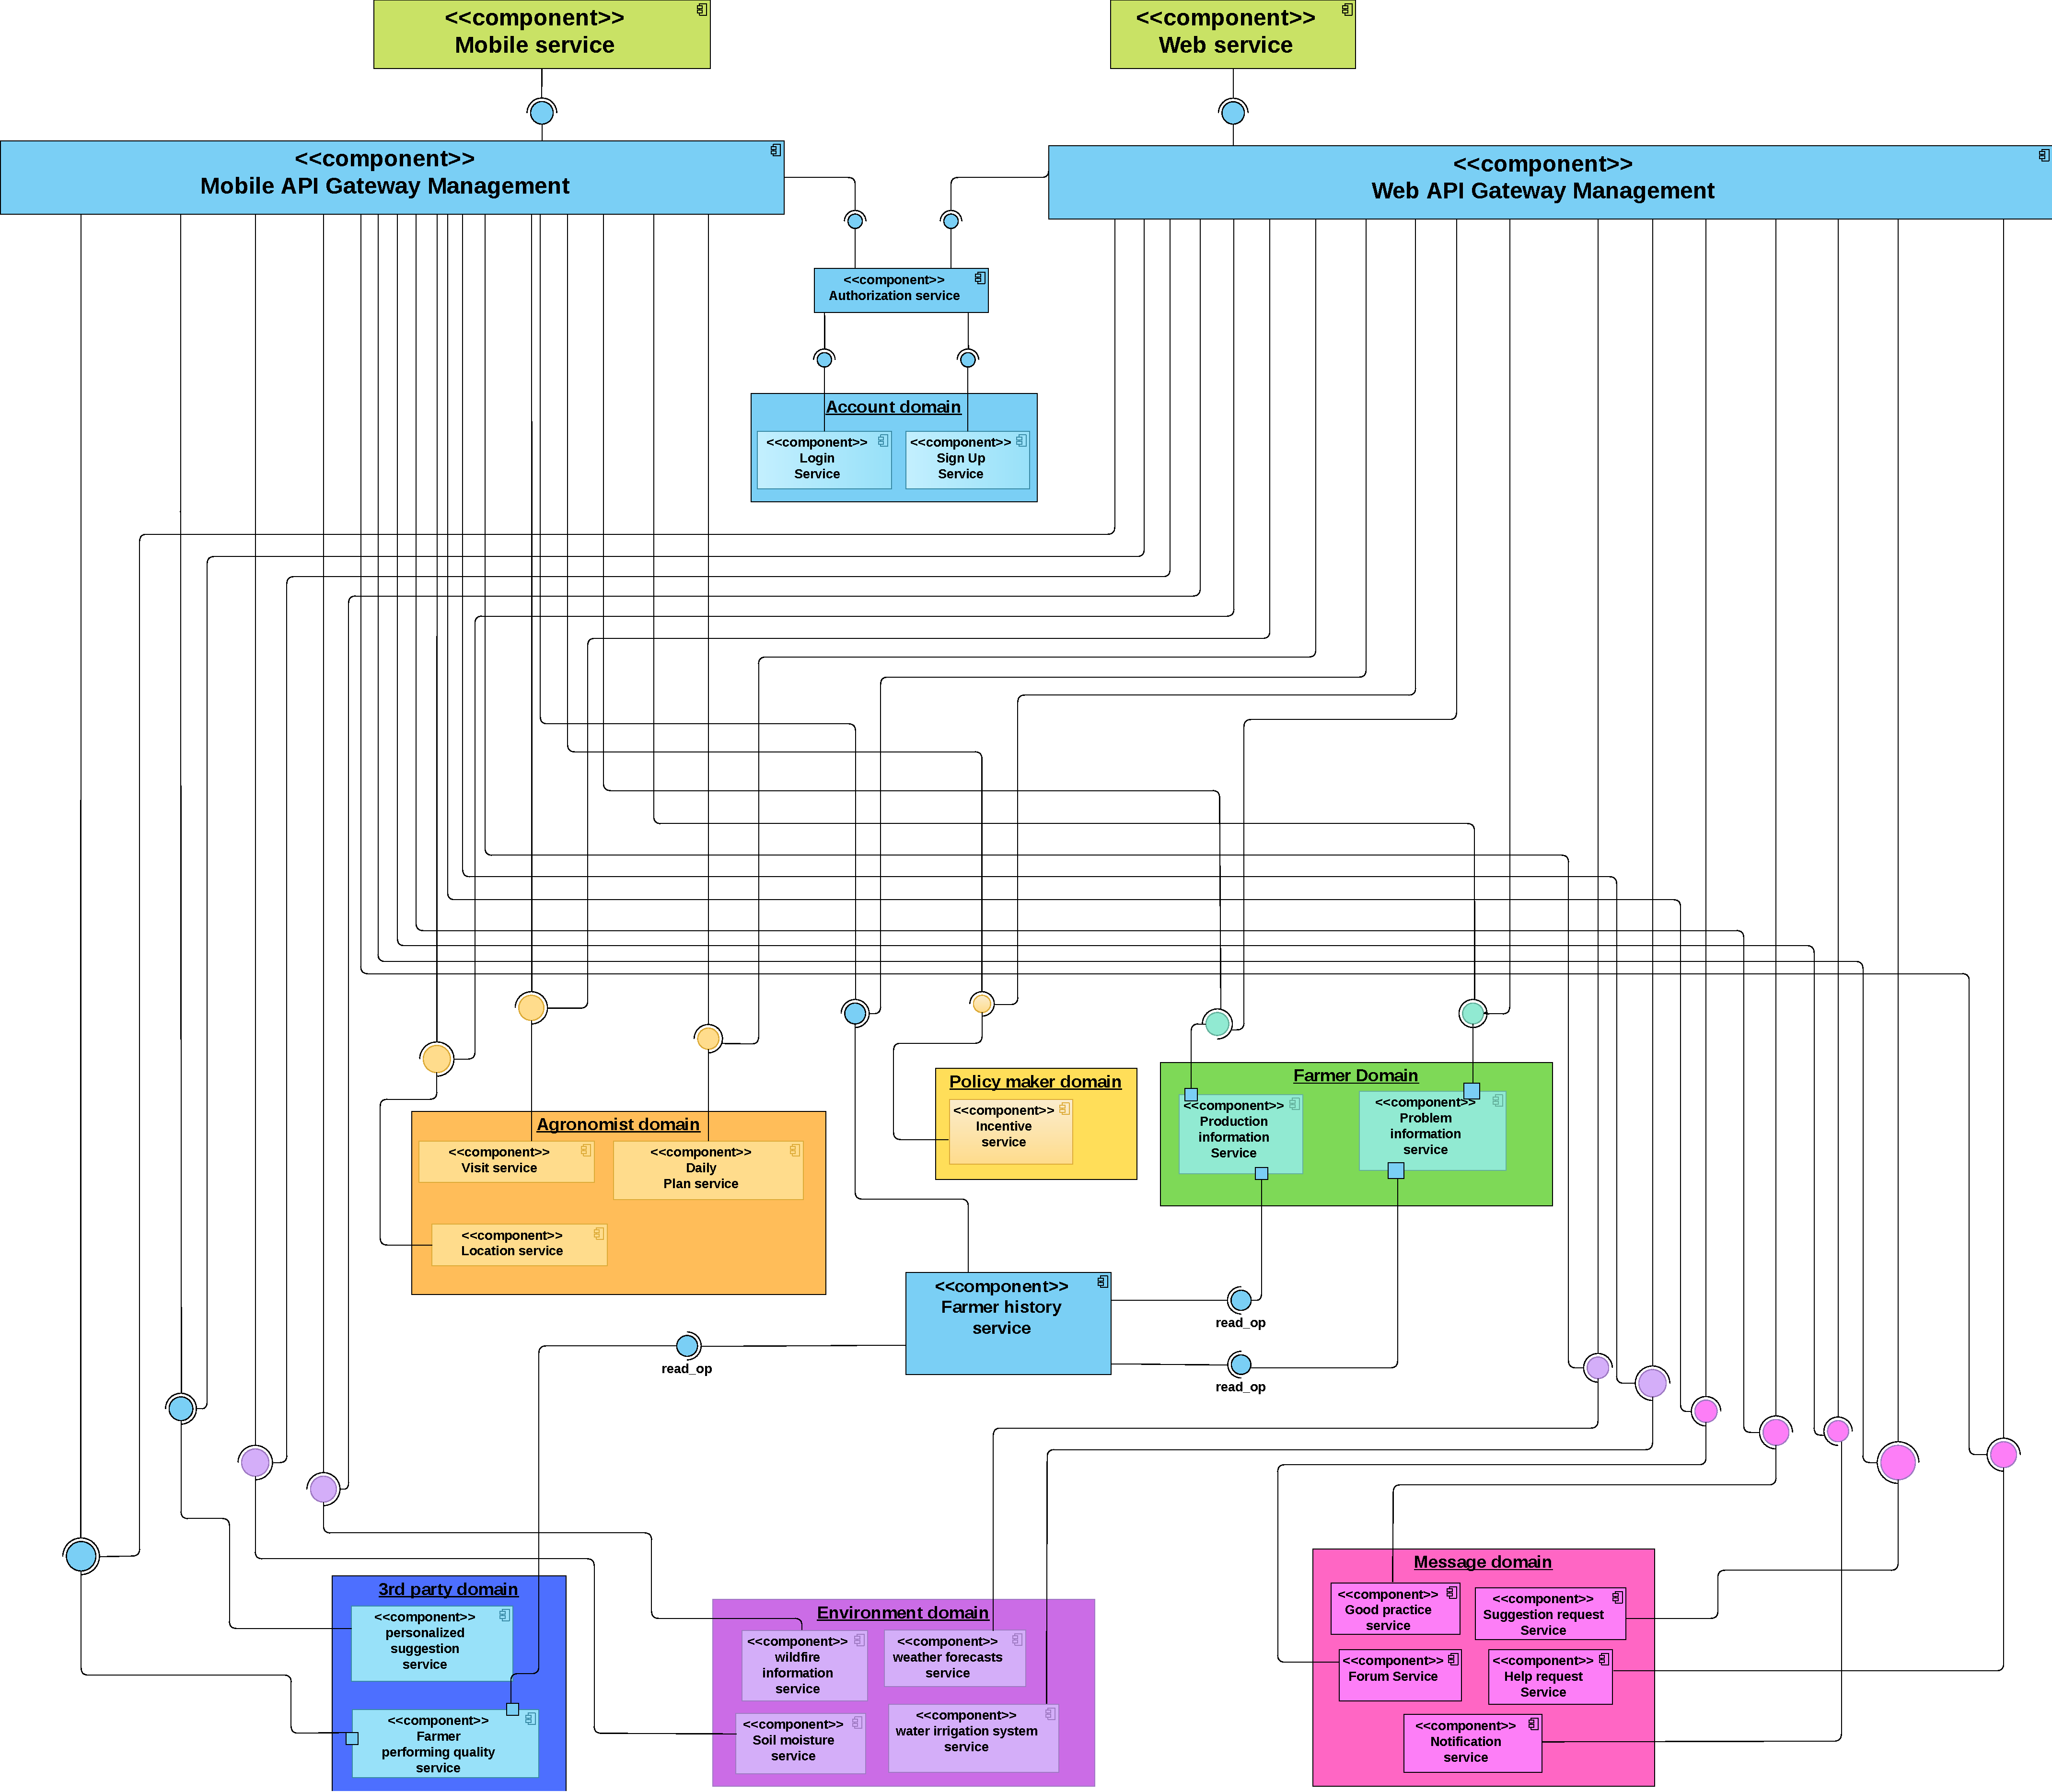
\includegraphics[width=0.99\paperwidth]{Images/Component Diagram2.pdf}}
    \caption{\label{fig:component_diagram}Component diagram}
\end{figure}

In figure \ref{fig:component_diagram} the platform is decomposed in 7 main domains:
\begin{itemize}
    \item The \textsc{\textcolor{cyan}{Account}} Domain contains all the features in order to manage the user side. In fact, it includes the log in and sign up micro-services. Moreover, the component provides different interfaces for different users, in order to provide additional distinct information.
    \item The \textsc{\textcolor{pink}{Message}} domain handles all different kind of message information exchanged between users, from simplest suggestion and help requests to forum and good practice document requests. These micro-services are completely used by farmers, and partially used by both agronomists and policy makers.
    \item The \textsc{\textcolor{purple}{Legacy}} domain contains micro-services that handle all the available environment information gathered by sensors along the state of Telangana. The four micro-services contained in this domain manage the information of the water irrigation system, of the soil moisture, of the weather forecasts and the wildfire ones.
    \item The \textsc{\textcolor{blue}{3rd Party}} domain provides statistics mainly based on farmers information and the integration with the environment service information. This module is composed by two micro-services responsible to provide reliable farmer's performance quality information and personalized suggestion.
    \item The \textsc{\textcolor{green}{Farmer}} domain contains farmer related CQRS-based micro-services providing CRUD operations for production and problem information.
    \item The \textsc{\textcolor{orange}{Agronomist}} domain contains those micro-services that fulfill agronomist requirements. In particular they provide utilities for managing the area they are responsible of, for the daily plan and for the visits confirmation.
    \item The \textsc{\textcolor{yellow}{Policy maker}} domain is composed by a single main micro-service that is responsible to provide the incentive assignment functionality.
    \item Finally the Farmer history micro-service provides READ only operations. This component uses event handlers that subscribe to events published by Farmer and 3rd party domains' services in order to keep its database updated.
\end{itemize}


% Micro-service integration is not anymore based on \textit{Enterprise Service Bus} (ESB) but they rely on \textit{smart endpoints and dumb pipes} style.

% source: https://medium.com/@nathankpeck/microservice-principles-smart-endpoints-and-dumb-pipes-5691d410700f